\chapter{Effects and Animations}

Up until this chapter we have built a fully functional game that could be
shipped to the App Store! This last chapter will deal with polishing the game and making
it more delightful. \SB{} and \cocos{} provide powerful, yet simple to use tools
to create visual effects and animations. In this chapter we will add light
effects and we'll use the \SB{} timeline to bring some more motion to our
gameplay.

\section{Lighting with CCEffects}
Let's start by adding some light effects to our game. Lighting effects can make
a game feel a lot more polished. Here's a comparison of what our game looks like
right now, and how it will look once we're completed this section:

\begin{figure}[H]
    \centering
    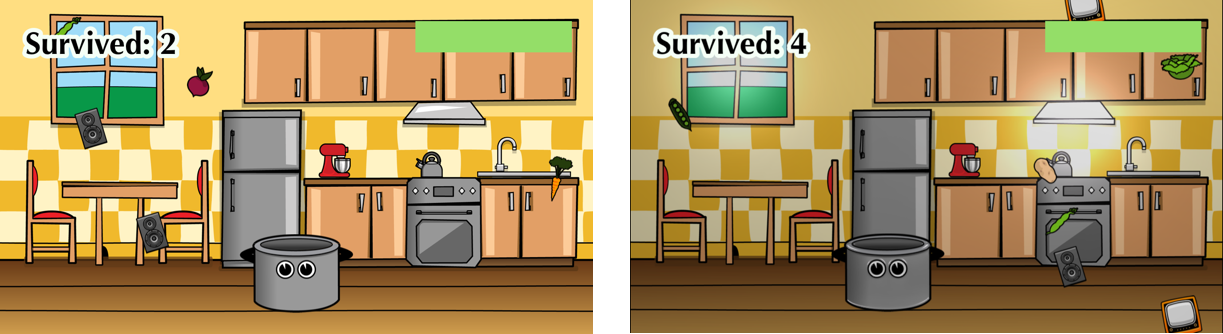
\includegraphics[width=0.9\linewidth]{images/Chapter9/lighting_comparison.png}
    \caption{Unlighted scene on the left, lighted scene on the right}
    \label{lighting_example}
\end{figure}

Most game engines require developers to write \textit{shader programs} to
use visual effects such as lighting. \cocos{} provides an API called
\inlinecode{CCEffects} that implements many common visual effects, such as
lighting, refraction, blur, etc. Using CCEffects we can enhance our games
without needing to learn how to write shader programs. 

The CCEffects can even be configured with \SB{}! We can set up all of the
lighting for this game with only a handful lines of code. 

The first step of adding lighting to our game is understanding some of the
theory that goes into lighting in 2D games.

\subsection{Lighting in 2D games}
The simplest way to light a 2D scene is to use brighter and darker colors,
depending on the distance to a given light source, I'll refer to this technique
as \textit{flat lighting}. Figure \ref{lighting_example} shows flat lighting on
the background image of our game. Some areas of the background are lighter than
others. The background is the lightest around the window and the kitchen light,
the two light sources for our game.

Flat lighting comes entirely out of the box using \cocos{}. However, using flat
lighting alone doesn't create great visual effects. In 2D games lighting can be
used to give objects a 3D feel. We are going to use that technique for the pot
and the falling objects.

We will create \textit{normal maps} for each of our game objects. A normal map
is a special kind of texture that describes the 3D surface of an object. That
way the game engine can calculate how strong certain areas of a texture should
be light up by a light source. Here's what a normal map looks like:

\begin{figure}[H]
    \centering
    
\includegraphics[width=180pt]{images/Chapter9/pot-bottom_NRM.png}
    \caption{The normal map for the bottom part of the pot. Each color encodes
    information about the object's surface}
\end{figure}

And here's a comparison that shows how lighting and normal maps together give
the pot a 3D feel:

\begin{figure}[H]
    \centering
    
\includegraphics[width=300pt]{images/Chapter9/pot_lighting_comparison.png}
    \caption{No lighting on the left, lighting with normal map on the right}
\end{figure}

The comparison above shows that certain parts of the pot appear brighter and
shinier. \cocos{} calculates the brightness for each part of the texture based
on the normal map that we provide and the position of the light. 

Lighting and normal maps for 2D games are topics that are worth dedicating
entire books to (and there are a ton out there!) so for now we will stick with
this overview of how lighting works. Even this basic knowledge will allows us to
make the game look quite a bit better. You might wonder where the normal maps
for our textures come from. The answer is: we need to create them ourselves. 

\subsection{Creating normal maps}
There are a bunch of tools available that turn creating simple normal maps into
an easy task. For this book I've provided all of the normal maps for you, as
part of the asset pack that you downloaded at the beginning of this book.

%TODO: check crazy bump license
What if you want to create normal maps for your own game? The normal maps for
this book have been created with the tool \textit{CrazyBump}
(\url{http://www.crazybump.com/}). CrazyBump uses shape detection to guess
normal maps and the results have been great for me!

If you have complicated textures, or you need to polish the lighting effects in
your game in great detail, you might want to resort to a tool that allows you to
create a normal map manually. \textit{SpriteIlluminator}
(\url{https://www.codeandweb.com/spriteilluminator}) is a great tool for
manually creating normal maps.

Since we already have all the normal maps we need, let's dive right into \SB{}
and set up some light sources!

\subsection{Setting up lighting effects in \SB{}}
Now that we have a basic understanding of 2D lighting it's time to dive into the
CCEffects API. There are three important components that we will be using:
\begin{description}
\item[CCEffectNode] is a container for all visual effects. If
you want to apply effects to \ccsprite{}s, all of them need to be the child of a
\inlinecode{CCEffectNode}. In practice this means that you'll mostly have a
\inlinecode{CCEffectNode} as a container for your entire gameplay scene.
\item[CCEffect] represents one of the different available visual effects, e.g.
lighting, refraction, blur, etc. Currently effects can only be applied to
\ccsprite{}s. You add an effect to a sprite by instantiating a
\inlinecode{CCEffect} and assigning it to a \ccsprite{}.
\item[CCLightNode] is used in combination with the effect
\inlinecode{CCEffectLighting} to define light sources.
\end{description}

To summarize what we've dicussed so far: Effects can only be applied to
\ccsprite{}s. All affected sprites need to be a child of a
\inlinecode{CCEffectNode}. Light nodes are used together with the lighting
effect and define light sources. Direction and brightness of these light nodes
is used by \cocos{} to render lighting effects.

Here's a diagram of how the components play together:

\begin{figure}[H]
    \centering
    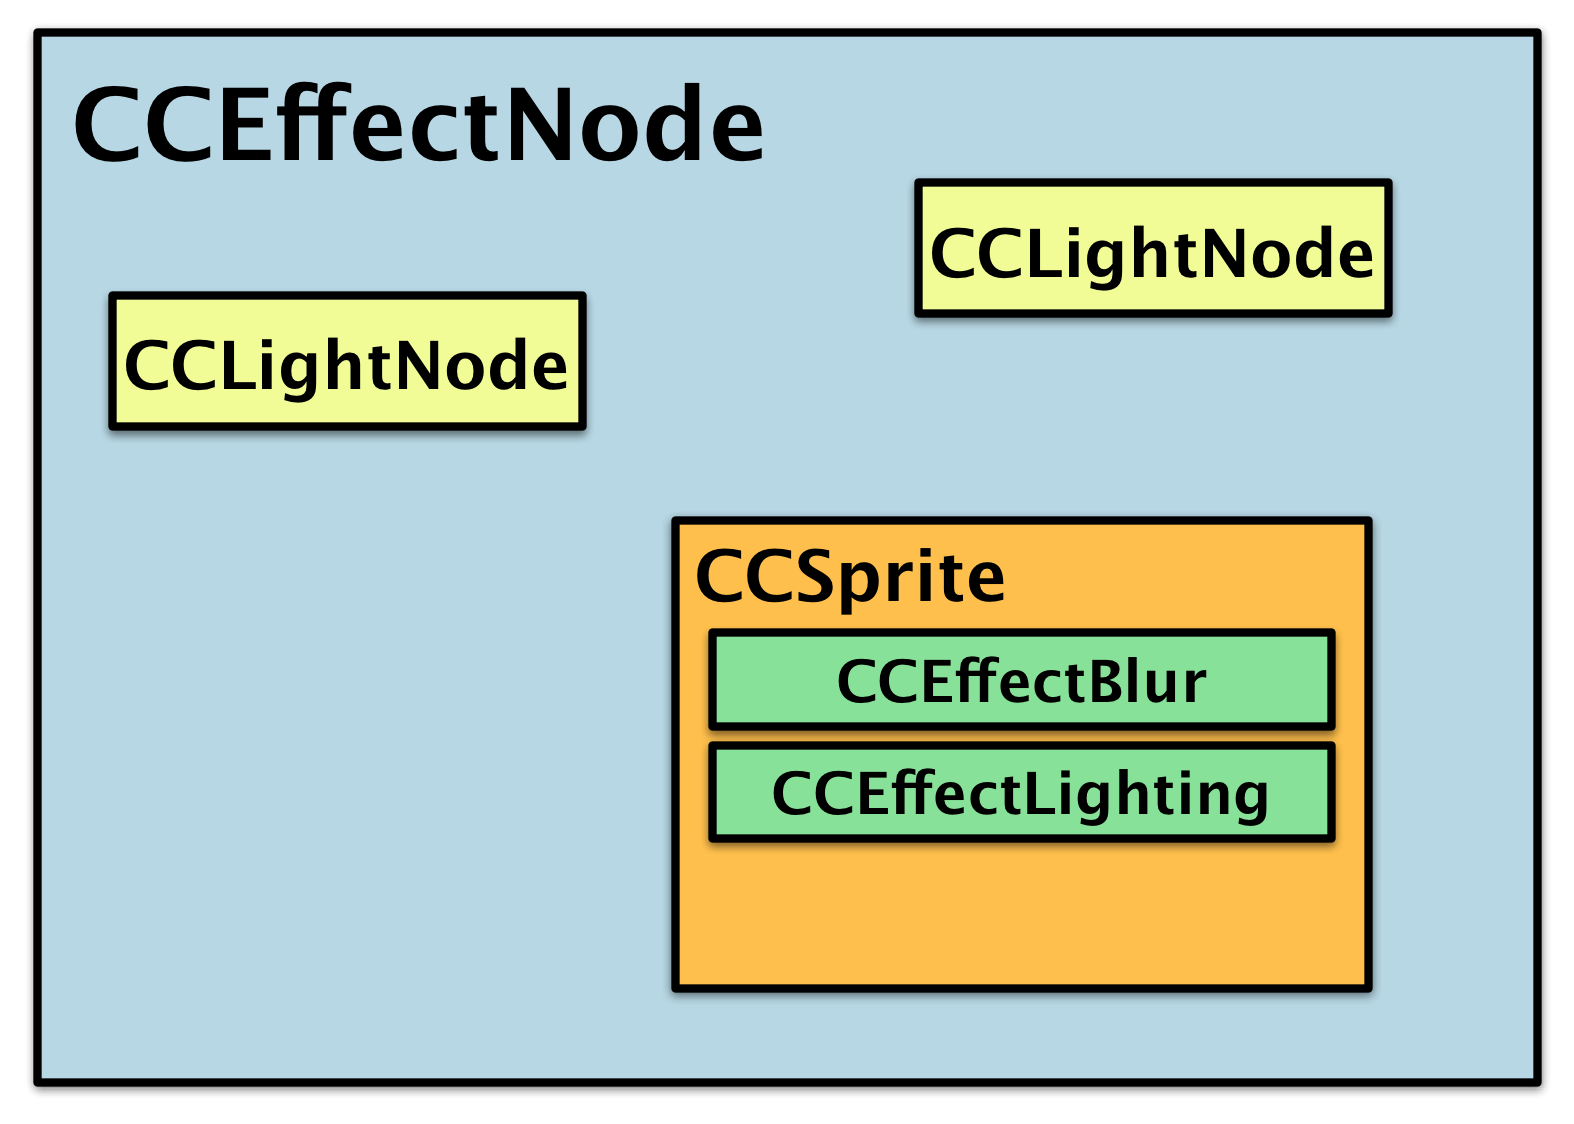
\includegraphics[width=260pt]{images/Chapter9/effect_setup.png}
\end{figure}

We will only discuss a subset of the \inlinecode{CCEffects} API, but the good
news is that it is very easy to use and therefore can be explored without much
instruction! 

There a many simple effects that can be added with a single line of
code, such as \textit{blur} or \textit{saturation}. You can add all effects in
code or in \SB{}. You can change the relevant
properties of a \inlinecode{CCEffect} in code, that
alows you to animate effects. You can for example create
a \textit{saturation} effect that starts with full
saturation and over time reduces the saturation until
the sprite turns into a grayscale image.

Finally, \inlinecode{CCEffectStack} allows you to
combine multiple effects.

\begin{details}[frametitle={More on effects}]
If you want to learn a little bit more about effects in \cocos{} you should read
our tutorial that introduces the \inlinecode{CCEffects} 
API (\url{https://www.makeschool.com/tutorials/cocos2d-3-2-with-cceffects-is-coming}).
\end{details}

This introduction gives us enough understanding to move to \SB{} and set up our
lighting. Open the \SB{} project and select the \filemention{MainScene.ccb}
file.

\begin{leftbar}
\begin{enumerate}
  \item Drag an \textit{Effect Node} from the node library to the timeline of
  \filemention{MainScene.ccb}
  \item Use the {Shift} key to select all of the nodes that are currently added
  to Main Scene: \begin{figure}[H]
    \centering
    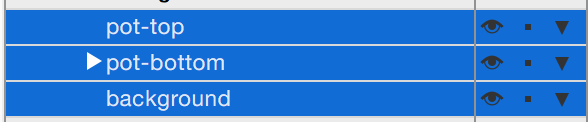
\includegraphics[width=200pt]{images/Chapter9/shift_select.png}
    \end{figure}
  \item Drag the selected nodes onto the \textit{Effect Node} to turn all of the nodes into children of the effect node. Your node
  hierarchy should look like this:
  \begin{figure}[H]
    \centering
    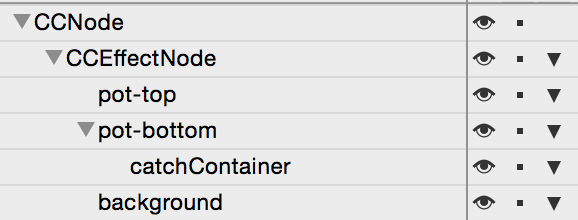
\includegraphics[width=200pt]{images/Chapter9/node_hierarchy_effect.png}
  \end{figure}
  \item Set the content size of the effect node to \textit{percentage of parent
  container} and set the size to (100\%, 100\%)
\end{enumerate}
\end{leftbar}

Now we have the \inlinecode{CCEffectNode} set up, which allows us to add visual
effects!

\subsection{Assigning normal maps in code}